\documentclass[pdftex,francais]{beamer}

% Copyright 2004 by Till Tantau <tantau@users.sourceforge.net>.
%
% This file can be redistributed and/or modified under
% the terms of the GNU Public License, version 2.

%% \ifx\themename\undefined
%%   \def\themename{default}
%% \fi

\usetheme{lama}
%\usetheme{Madrid}
%\usecolortheme{crane}

\usepackage{multirow}
\usepackage[latin1]{inputenc}           %%%  
\usepackage[T1]{fontenc}                %%%
\usepackage[francais]{babel}            %%%

\usepackage{multimedia}
\usepackage{hyperref}
\usepackage{tikz}
\usepackage{listings}

%\newtheorem{theorem}{Th�or�me}

%\setbeamercovered{transparent}

\title[Irreducible fractions, patterns and straightness in DGtal]{Irreducible fractions, patterns and straightness\\
  DGtal, Arithmetic package (since 0.5)
}

\author[J.-O. Lachaud]{Jacques-Olivier Lachaud}

\date{DGtal Meeting, june 2012}


\graphicspath{{Figures/},{Images/}}

%%% \AtBeginSection[]
%%% {
%%%   \begin{frame}<beamer>
%%%     \frametitle{Plan}
%%%     \tableofcontents[currentsection] %,currentsubsection]
%%%   \end{frame}
%%% }


\renewcommand{\vec}[1]{\mathbf{#1}}

% space of the real numbers
\newcommand{\R}{\ensuremath{\mathbb{R}}}
% space of the integer numbers
\newcommand{\Z}{\ensuremath{\mathbb{Z}}}
% Digitization process of step h (1)
\newcommand{\Dig}[1]{\ensuremath{\mathrm{Dig}_{#1}}}
% Family of shape
\newcommand{\SF}[0]{\ensuremath{\mathbb{F}}}
% Topological boundary of X (1).
\newcommand{\TB}[1]{\ensuremath{\partial #1}}
% Discrete geometric estimator of G (1)
\newcommand{\DGE}[1]{\ensuremath{E_{#1}}}
% Reference shape of digital object O (1) with grid step $h$ (2).
\newcommand{\RS}[2]{\ensuremath{R_{#1,#2}}}

% Digital contour.
\newcommand{\DC}{\ensuremath{C}}
% Continuous contour.
\newcommand{\CC}{\ensuremath{\mathcal{C}}}
% A point indexed by i (1) on the digital contour.
\newcommand{\PT}[1]{\ensuremath{\DC_{#1}}}
% A sequence of points indexed by i (1) on the digital contour.
\newcommand{\PTS}[2]{\ensuremath{\DC_{#1,#2}}}
% Predicate stating that the digital curve is a segment between indices 1 and 2
\newcommand{\SPRED}[2]{\ensuremath{S(#1,#2)}}
% ET logique
\newcommand{\AND}[0]{\ensuremath{\wedge}}
% OU logique
\newcommand{\OR}[0]{\ensuremath{\vee}}

% Tangent direction mapping of curve C (1)
\newcommand{\TGT}[1]{\ensuremath{\theta_{#1}}}
% Integral of squared curvature of curve C (1)
\newcommand{\ISC}[1]{\ensuremath{J[#1]}}
% Smallest possible tangent direction at constraint l (1)
\newcommand{\MinTD}[1]{\ensuremath{a_{#1}}}
% Largest possible tangent direction at constraint l (1)
\newcommand{\MaxTD}[1]{\ensuremath{b_{#1}}}
% Unknown tangent direction at constraint l (1)
\newcommand{\UnkTD}[1]{\ensuremath{t_{#1}}}

% ideal multiscale criterion
\newcommand{\IMSC}[2]{\ensuremath{\mu_{#1}(#2)}}
% multiscale profile
\newcommand{\MSP}[2]{\ensuremath{\mathcal{P}_{#1}(#2)}}
% threshold flat/curve
\newcommand{\CThreshold}[0]{\ensuremath{t_{f/c}}}
% threshold noise
\newcommand{\NThreshold}[0]{\ensuremath{t_{m}}}
% noise level
\newcommand{\NL}[0]{\ensuremath{\nu}}
% slope linear regression 
\newcommand{\SLR}[2]{\ensuremath{\theta_{#1}}}





% Pencil of maximal segments around a point.
\newcommand{\PE}[1]{\ensuremath{{\mathcal P}(#1)}}
% Tangent orientation of the maximal segment.
\newcommand{\TO}[1]{\ensuremath{\theta_#1}}
% lambda function for interpolation.
\newcommand{\LF}{\ensuremath{\lambda}}
% \lambda-MS tangent orientation.
\newcommand{\LTO}[1]{\ensuremath{\hat{\theta}(#1)}}
% \lambda-MS tangent orientation variation.
\newcommand{\LTOP}[1]{\ensuremath{\hat{\theta}'(#1)}}

%\definecolor{rougeSW_}{rgb}{0.968627,0.011765,0.015686}
\definecolor{darkgreen}{rgb}{0.0,0.6,0.0}
\definecolor{lightblue}{rgb}{0.5,0.5,1.0}
\definecolor{magenta}{rgb}{1.0,0.0,1.0}
\newcommand{\alertred}[1]{{\color{red}#1}}
\newcommand{\Cb}[1]{{\color{blue}#1}}
\newcommand{\Cdg}[1]{{\color{darkgreen}#1}}
\newcommand{\textmagenta}[1]{{\color{magenta}#1}}
\newcommand{\Implies}{{\ensuremath{\Rightarrow}}}

\newcommand{\Refs}[1]{{\color{lightblue}#1}}
\newcommand{\Cite}[1]{\Refs{[#1]}}
\newcommand{\Etal}{{\em et al.}}
\newtheorem{remark}{Remarque}
% Digitization process of step h (1)
\newcommand{\DigGh}[2]{\ensuremath{\mathrm{Dig}_{#2}(#1)}}
\newcommand{\BigT}{\ensuremath{\Theta}}
\newcommand{\BigO}{\ensuremath{O}}

\newcommand{\TAN}[0]{\ensuremath{\theta}}
% Position estimator
\newcommand{\EPOS}[0]{\ensuremath{\hat{{x}}}}
% Convexity Position estimator 
\newcommand{\ECONVPOS}[0]{\ensuremath{\hat{x}^\mathrm{conv}}}
% tangent estimator base MS.
\newcommand{\ETANMS}[0]{\ensuremath{\hat{\TAN}^{\text{MS}}}}
% tangent estimator base arete du CDP.
\newcommand{\ETANEDGE}[0]{\ensuremath{\hat{\TAN}^{\text{conv}}}}
% estimateur de longueur elementaire d'un surfel (1) sur le bord discretise de X(2) de pas h(3).

\newcommand{\Class}[1]{\alert{\texttt{#1}}}
\newcommand{\Concept}[1]{\texttt{\color{magenta}#1}}
\newcommand{\Method}[1]{\texttt{\color{lightblue}#1}}


\definecolor{MyGreen}{rgb}{0,0.6,0}

\setbeamercolor{qcolorb}{fg={blue!20!black},bg={blue!15!white}}
\setbeamercolor{qcolorub}{fg={blue!10!black},bg={blue!30!white}}
\setbeamercolor{qcolorlb}{fg={blue!20!black},bg={blue!8!white}}
\setbeamercolor{qcolorulb}{fg={blue!10!black},bg={blue!40!white}}
\setbeamercolor{qcolorg}{fg={green!20!black},bg={green!15!white}}
\setbeamercolor{qcolorug}{fg={green!10!black},bg={green!30!white}}
\setbeamercolor{qcolorlg}{fg={green!20!black},bg={green!8!white}}
\setbeamercolor{qcolorulg}{fg={green!10!black},bg={green!40!white}}
\setbeamercolor{qcolorr}{fg={red!20!black},bg={red!15!white}}
\setbeamercolor{qcolorur}{fg={red!10!black},bg={red!30!white}}
\setbeamercolor{qcolorlr}{fg={red!20!black},bg={red!8!white}}
\setbeamercolor{qcolorulr}{fg={red!10!black},bg={red!40!white}}
\newenvironment{myblockbluish}[2]%
	       {\begin{beamerboxesrounded}[lower=qcolorb,upper=qcolorub,width=#1,shadow=true]{#2}}{\end{beamerboxesrounded}}
\newenvironment{myblocklbluish}[2]%
	       {\begin{beamerboxesrounded}[lower=qcolorlb,upper=qcolorulb,width=#1,shadow=true]{#2}}{\end{beamerboxesrounded}}
\newenvironment{myblockgreenish}[2]%
	       {\begin{beamerboxesrounded}[lower=qcolorg,upper=qcolorug,width=#1,shadow=true]{#2}}{\end{beamerboxesrounded}}
\newenvironment{myblocklgreenish}[2]%
	       {\begin{beamerboxesrounded}[lower=qcolorlg,upper=qcolorulg,width=#1,shadow=true]{#2}}{\end{beamerboxesrounded}}
\newenvironment{myblockredish}[2]%
	       {\begin{beamerboxesrounded}[lower=qcolorr,upper=qcolorur,width=#1
,shadow=true]{#2}}{\end{beamerboxesrounded}}
\newenvironment{myblocklredish}[2]%
	       {\begin{beamerboxesrounded}[lower=qcolorlr,upper=qcolorulr,width=#1,shadow=true]{#2}}{\end{beamerboxesrounded}}

%%%%%%%%%%%%%%%%%%%%%%%%%%%%%%%%%%%%%%%%%%%%%%%%%%%%%%%%%%%%%%%%%%%%%%%%%%%%%%%
%%%%%%%%%%%%%%%%%%%%%%%%%%%%%%%%%%%%%%%%%%%%%%%%%%%%%%%%%%%%%%%%%%%%%%%%%%%%%%%
%%%%%%%%%%%%%%%%%%%%%%%%%%%%%%%%%%%%%%%%%%%%%%%%%%%%%%%%%%%%%%%%%%%%%%%%%%%%%%%
  \lstset{language=c++, numbers=left, tabsize=2, frame=single, breaklines=true, basicstyle=\ttfamily\scriptsize,
     numberstyle=\tiny\ttfamily, framexleftmargin=13mm, xleftmargin=12mm,keywordstyle=\color{blue}\bfseries,%
     commentstyle=\sffamily\color{red}}

\begin{document}

\newlength{\unquart}
\setlength{\unquart}{0.21\textwidth}

%------------------------------------------------------------------------------
\begin{frame}
  \titlepage
\end{frame}
%------------------------------------------------------------------------------

%%%%%%%%%%%%%%%%%%%%%%%%%%%%%%%%%%%%%%%%%%%%%%%%%%%%%%%%%%%%%%%%%%%%%%%%%%%%%%%
\section{Introduction}
%%%%%%%%%%%%%%%%%%%%%%%%%%%%%%%%%%%%%%%%%%%%%%%%%%%%%%%%%%%%%%%%%%%%%%%%%%%%%%%

%------------------------------------------------------------------------------
\begin{frame}%[allowframebreaks]
  \frametitle{Arithmetic package content}

  \begin{myblocklbluish}{\textwidth}{Content (\alertred{New} package in DGtal 0.5)}
    \begin{itemize}
    \item elementary integer arithmetic algorithms (gcd, B�zout)
    \item several representations for irreducible fractions
      \begin{itemize}
      \item Stern-Brocot tree
      \item continued fractions
      \item rational approximations
      \end{itemize}
    \item patterns
    \item digital straight lines and subsegments
    \end{itemize}
  \end{myblocklbluish}

  \begin{myblocklredish}{\textwidth}{Location}
    \begin{itemize}
      \small
    \item \texttt{\{DGtal\}/src/DGtal/math/arithmetic}
    \item \texttt{\{DGtal\}/tests/math/arithmetic}
    \item \texttt{\{DGtal\}/examples/math/arithmetic}
    \end{itemize}
  \end{myblocklredish}

\end{frame}
%------------------------------------------------------------------------------

%%%%%%%%%%%%%%%%%%%%%%%%%%%%%%%%%%%%%%%%%%%%%%%%%%%%%%%%%%%%%%%%%%%%%%%%%%%%%%%
\section{Elementary arithmetic}
%%%%%%%%%%%%%%%%%%%%%%%%%%%%%%%%%%%%%%%%%%%%%%%%%%%%%%%%%%%%%%%%%%%%%%%%%%%%%%%

%------------------------------------------------------------------------------
\begin{frame}[fragile]%[allowframebreaks]
  \frametitle{Elementary arithmetic over arbitrary integer types}

  Class \href{http://liris.cnrs.fr/dgtal/doc/nightly/classDGtal_1_1IntegerComputer.html}{\texttt{\alertred{IntegerComputer}$<$Int$>$}}

  \begin{itemize}
  \item stores temporary variables (useful for {\tt BigInteger})
  \item elementary operations: max, min, abs, isPositive, ...
  \item provides classical arithmetic computations: gcd, extended
    Euclid, convergents, continued fraction
  \end{itemize}

  \lstset{language=c++, numbers=left, tabsize=2, frame=single, breaklines=true, basicstyle=\ttfamily\tiny,
     numberstyle=\tiny\ttfamily, framexleftmargin=13mm, xleftmargin=12mm,keywordstyle=\color{blue}\bfseries,%
     commentstyle=\sffamily\color{red}}
  \lstset{emph={gcd,extendedEuclid,getCFrac},emphstyle=\color{MyGreen}}

  \begin{lstlisting}
  typedef DGtal::BigInteger Integer;
  IntegerComputer<Integer> ic; // instance for computations
  Integer g = ic.gcd( 192, 128 ); // 64
  IntegerComputer<Integer>::Vector2I v
    = ic.extendedEuclid( 5, 12, 2 ); // solution to 5x+12y = 2
  std::cout << "5x+12y=2 <=> x=" << v[0] 
	    << " y=" << v[1] << std::endl; // 5x+12y=2 <=> x=10 y=-4
  std::vector<Integer> q; // quotients
  ic.getCFrac( q, 5, 13 ); // continued fraction
  std::cout << "5/13=[" << q[0] << ";" << q[1] 
	    << "," << q[2] << "," << q[3]
	    << "," << q[4] << "]" << std::endl; // 5/13=[0;2,1,1,2]
   \end{lstlisting}
  \begin{itemize}
  \item[$+$] more complex operations related to integer half spaces
  \end{itemize}
\end{frame}

%------------------------------------------------------------------------------
\begin{frame}[fragile]%[allowframebreaks]
  \frametitle{Elementary arithmetic over arbitrary integer types (II)}
  \lstset{language=c++, numbers=left, tabsize=2, frame=single, breaklines=true, basicstyle=\ttfamily\tiny,
     numberstyle=\tiny\ttfamily, framexleftmargin=13mm, xleftmargin=12mm,keywordstyle=\color{blue}\bfseries,%
     commentstyle=\sffamily\color{red}}
  \lstset{emph={gcd,extendedEuclid,getCFrac},emphstyle=\color{MyGreen}}
  \begin{lstlisting}
  ic.getCFrac( q, 
               Integer("51234567894643563456345635435722900123"), 
	       Integer("345678532087609239457759428901234" ) );
  std::cout << "[" << q[0];
  for ( unsigned int i = 1; i < q.size(); ++i )
    std::cout << "," << q[i];
  std::cout << "]" << std::endl;
  // [148214,2,29,3,3,1,1,1,8,2,5,1,4,3,4,1,1,2,1,1,2,1,1,2,1,5,1,1,
  //  4,2,2,1,1,1,4,3,2,1,1,2,3,1,2,3,1,14,1,3,13,7,1,1,1,1,1,9,1,1,
  //  27,3,1,1,3,8,1,1,1,8,6,1,1,2,6,3,1,1,4,4]
  \end{lstlisting}

\end{frame}

%%%%%%%%%%%%%%%%%%%%%%%%%%%%%%%%%%%%%%%%%%%%%%%%%%%%%%%%%%%%%%%%%%%%%%%%%%%%%%%
\section{Irreducible fractions}
%%%%%%%%%%%%%%%%%%%%%%%%%%%%%%%%%%%%%%%%%%%%%%%%%%%%%%%%%%%%%%%%%%%%%%%%%%%%%%%

%------------------------------------------------------------------------------
\begin{frame}[fragile]%[allowframebreaks]
  \frametitle{Properties of positive irreducible fractions}
  
  \begin{block}{Definition \alert{positive irreducible fraction}}
    \small A fraction $\frac{p}{q}$ with $p,q \in \Z^+, \gcd(p,q)=1$.
  \end{block}

  \begin{itemize}
  \item uniqueness, dense
  \item related to finite simple continued fractions (Euclid algorithm)
  \item generated by the Stern-Brocot tree
  \end{itemize}
\end{frame}
%------------------------------------------------------------------------------

%------------------------------------------------------------------------------
\begin{frame}[fragile]%[allowframebreaks]
  \frametitle{Simple continued fractions}

  \begin{block}{Definition \alert{simple continued fraction}}
    \scriptsize
    A number of the form $a_0+\cfrac{1}{a_1+\cfrac{1}{\ldots +
        \cfrac{1}{a_n}}}$, where $a_i$ are integers, commonly written
    as $[a_0;a_1,\ldots,a_n]$. The $a_i$ are the partial quotients.
  \end{block}
  \begin{itemize}
  \item \scriptsize Any simple continued fraction is a positive irreducible fraction
  \item \scriptsize Any positive irreducible fraction has two simple continued fraction representations
  \item \scriptsize use Euclid algorithm (\alertred{gcd}, \alert{quotients}), e.g. $\frac{5}{13}$.
    \scriptsize
    $\begin{array}{ccccccc}
       p & = & \alert{u} & * & q & + & r \\ \hline
       5 & = & \alert{0} & * & 13& + & 5 \\ 
      13 & = & \alert{2} & * & 5 & + & 3 \\
       5 & = & \alert{1} & * & 3 & + & 2 \\
       3 & = & \alert{1} & * & 2 & + & 1 \\
       2 & = & \alert{2} & * & \alertred{1} & + & 0 \\
  \end{array} \quad$ \raisebox{0.6cm}{$\frac{5}{13}=\alert{0}+\cfrac{1}{\alert{2}+\cfrac{1}{\alert{1}+\cfrac{1}{\alert{1}+\cfrac{1}{\alert{2}}}}}$}
  \end{itemize}
\end{frame}

%------------------------------------------------------------------------------
\begin{frame}[fragile]%[allowframebreaks]
  \frametitle{Convergents and approximation}

  \centerline{
    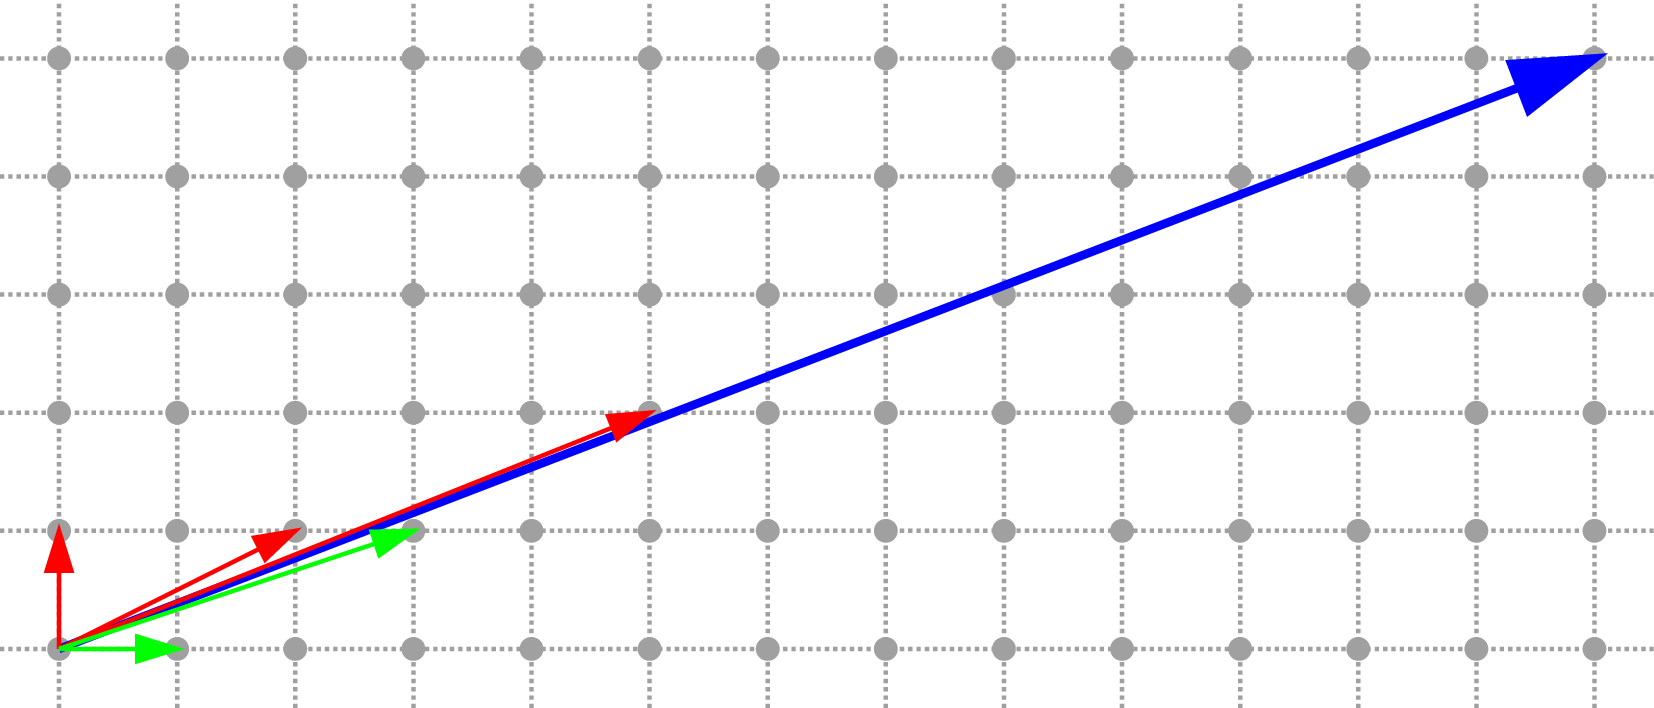
\includegraphics[width=0.7\textwidth]{approx-5-13}
  }

  \small
  {\color{blue} $z_4 = \frac{5}{13}=[0;2,1,1,2]$ }\\
  {\color{red} odd} convergents: 
  {\color{red} $z_3 = \frac{2}{5}=[0;2,1,1]$ }
  {\color{red} $z_1 = \frac{1}{2}=[0;2]$ }
  {\color{red} $z_{-1} = \frac{1}{0}=[]$ }\\
  {\color{green} even} convergents:
  {\color{green} $z_2 = \frac{1}{3}=[0;2,1]$ }
  {\color{green} $z_0 = \frac{0}{1}=[0]$ }

  \begin{itemize}
  \item convergents are the best approximations to fractions/real numbers
  \item thus related to digital straight lines
  \end{itemize}
\end{frame}
%------------------------------------------------------------------------------

%------------------------------------------------------------------------------
\begin{frame}[fragile]%[allowframebreaks]
  \frametitle{Stern-Brocot tree of irreducible fractions}

  \centerline{
    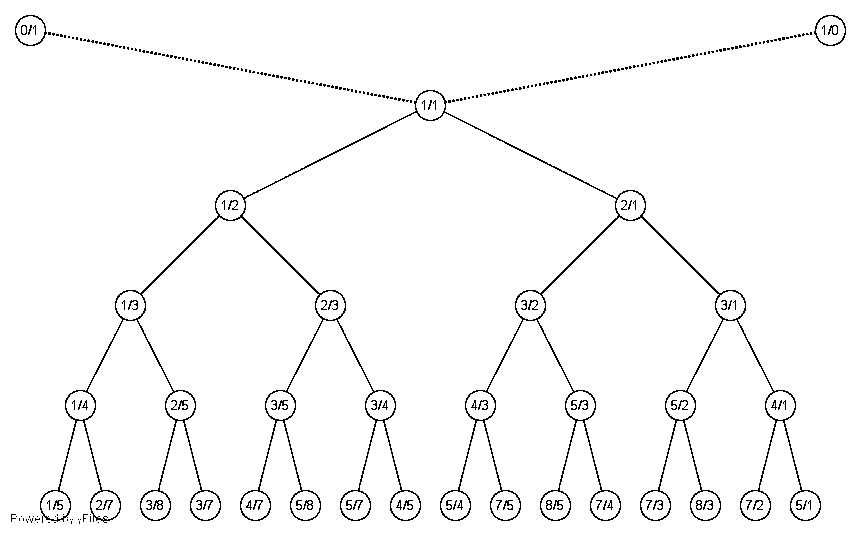
\includegraphics[width=0.8\textwidth]{Sternbrocot}
  }
  
  \begin{itemize}
  \item two starting fractions: $\frac{0}{1}$ and $\frac{1}{0}$
  \item mediant of two fractions: $\frac{p}{q} \oplus \frac{p'}{q'} = \frac{p+p'}{q+q'}$ (vector addition)
  \end{itemize}
  
\end{frame}


%------------------------------------------------------------------------------
\begin{frame}[fragile]%[allowframebreaks]
  \frametitle{Link with continued fractions}

  \centerline{
    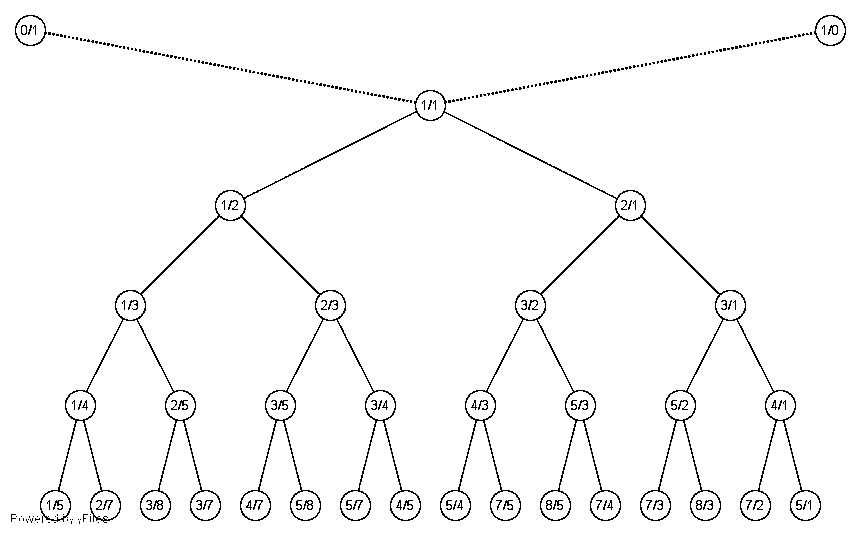
\includegraphics[width=0.8\textwidth]{Sternbrocot}
  }

  \begin{itemize}
  \item $u_0, u_1,\ldots, u_k $ = sequence of Right-then-Left moves from $\frac{1}{1}$, except last (one less).
  \item e.g. $\frac{5}{13}=[0;2,1,1,2]$, thus $R^0L^2RLR^{\alertred{2-1}}$.
  \end{itemize}
\end{frame}
%------------------------------------------------------------------------------

%------------------------------------------------------------------------------
\begin{frame}[fragile]%[allowframebreaks]
  \frametitle{Useful operations on fractions}
  
  \only<1-3>{
    \begin{itemize}
    \item if we forget $+$, $-$, $*$, $/$ ..., interesting operations are related to the ``tree'' structure
    \item making a fraction from its quotients, getting quotients
    \item mediant, left or right descendant, adding a quotient
    \item father, previous partial, $m$-father,
    \item arbitrary convergent / reduced partial
    \end{itemize}
  }

  \only<2>{
    \begin{block}{Requirements}
    \begin{itemize}
    \item Perform these operations in quasi-constant time !
    \item But storing quotients cost $O(\log(\max(p,q)))$
    \end{itemize}
    \end{block}
  }

  \only<3>{
  \begin{myblocklbluish}{\textwidth}{Solution}
    \begin{itemize}
    \item irreducible fraction described by concept \href{http://liris.cnrs.fr/dgtal/doc/nightly/structDGtal_1_1CPositiveIrreducibleFraction.html}{\texttt{\alertred{CPositiveIrreducibleFraction}}}
    \item explicit representation of the Stern-Brocot tree
    \item each node stores $k, u_k, p_k, q_k$
    \item but on-the-fly instanciation of nodes.
    \end{itemize}
  \end{myblocklbluish}
}
\end{frame}
%------------------------------------------------------------------------------

%------------------------------------------------------------------------------
\begin{frame}[fragile]%[allowframebreaks]
  \frametitle{Models of irreducible fractions (I)}

    \centerline{
      \only<1>{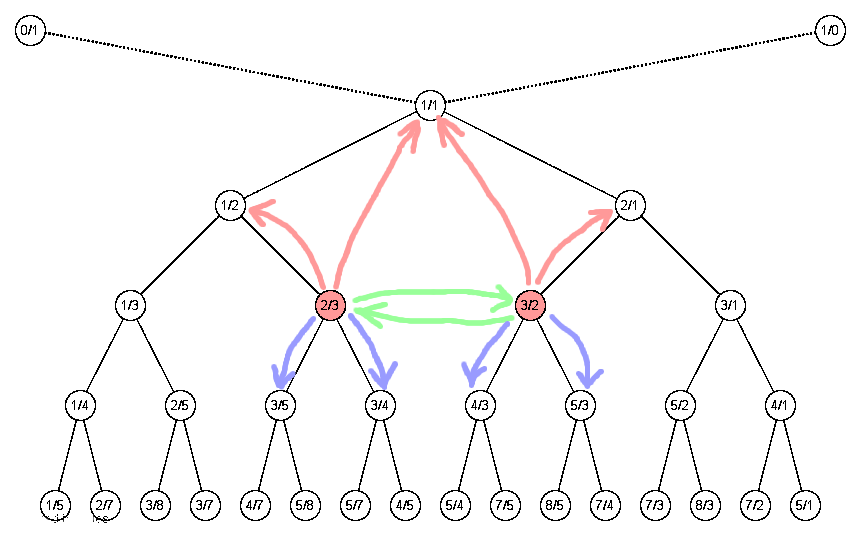
\includegraphics[width=0.7\textwidth]{Sternbrocot-2}}%
      \only<2>{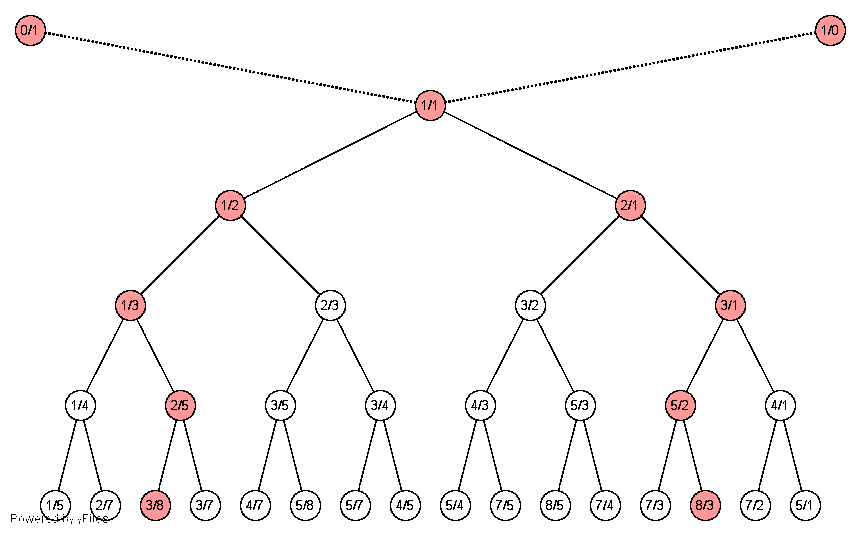
\includegraphics[width=0.7\textwidth]{Sternbrocot-nodes-5-13}}%
    }
  \small
  \begin{itemize}
  \item Class \href{http://liris.cnrs.fr/dgtal/doc/nightly/classDGtal_1_1SternBrocot.html}{\texttt{\alert{SternBrocot}}}, fraction is \texttt{SternBrocot::\alert{Fraction}}
  \item Each node knows 5 other nodes (fathers, reciprocal, direct descendants on demand)
  \item Simple, fast for small fractions, memory costly, operations in $O(u_k)$
  \end{itemize}


\end{frame}
%------------------------------------------------------------------------------

%------------------------------------------------------------------------------
\begin{frame}[fragile]%[allowframebreaks]
  \frametitle{Models of irreducible fractions (II)}

    \centerline{
      \only<1>{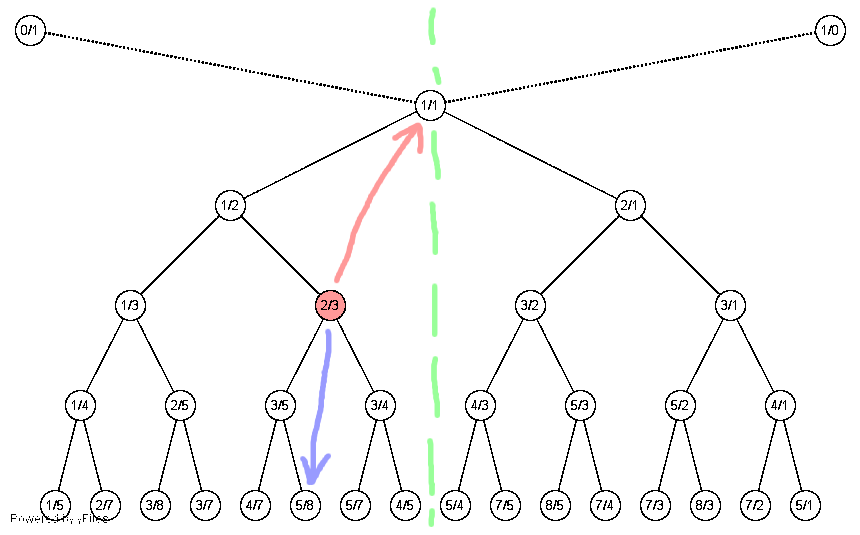
\includegraphics[width=0.7\textwidth]{LightSternbrocot}}%
      \only<2>{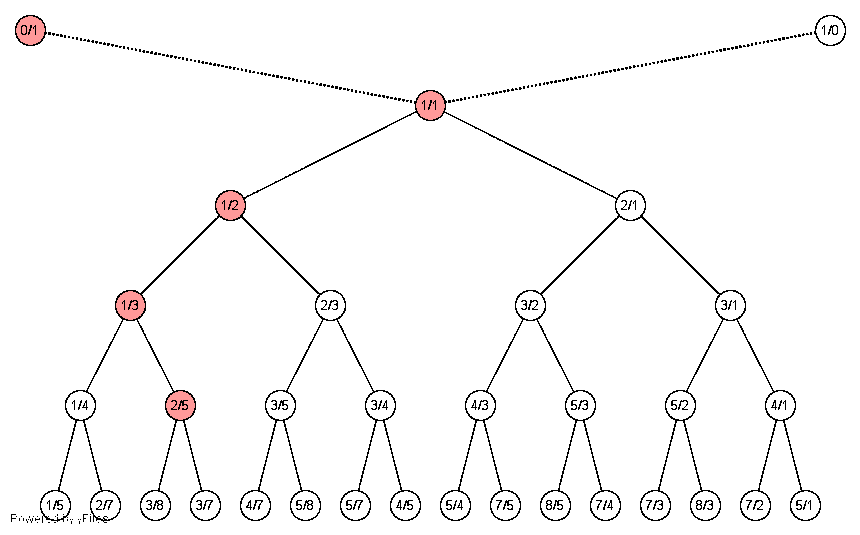
\includegraphics[width=0.7\textwidth]{LightSternbrocot-nodes-5-13}}%
    }
  \small
  \begin{itemize}
  \item Class \href{http://liris.cnrs.fr/dgtal/doc/nightly/classDGtal_1_1LightSternBrocot.html}{\texttt{\alert{LightSternBrocot}}}, fraction is \texttt{LightSternBrocot::\alert{Fraction}}
  \item Each node knows its reduced, mapping to next partials on demand
  \item fast for small fractions, less memory costly, but tricky cases
  \end{itemize}


\end{frame}
%------------------------------------------------------------------------------

%------------------------------------------------------------------------------
\begin{frame}[fragile]%[allowframebreaks]
  \frametitle{Models of irreducible fractions (III)}

    \centerline{
      \only<1>{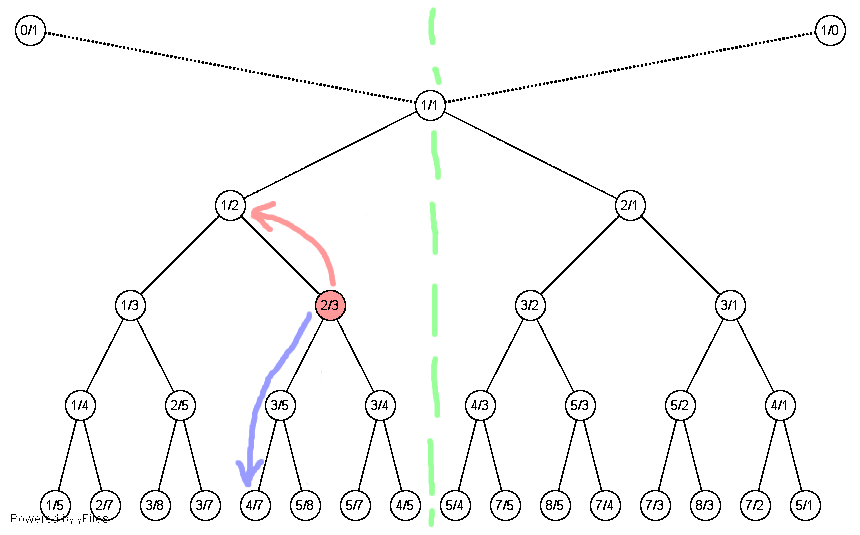
\includegraphics[width=0.7\textwidth]{LighterSternbrocot}}%
      \only<2>{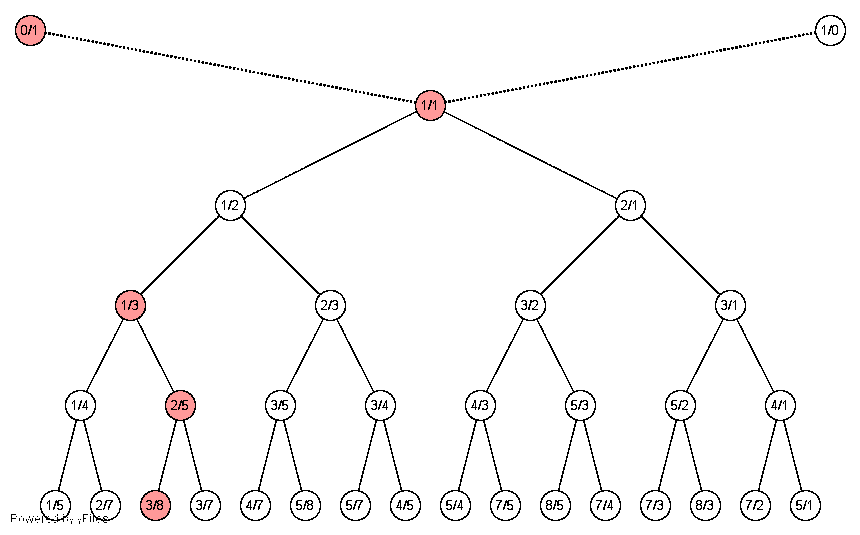
\includegraphics[width=0.7\textwidth]{LighterSternbrocot-nodes-5-13}}%
    }
  \small
  \begin{itemize}
  \item Class \href{http://liris.cnrs.fr/dgtal/doc/nightly/classDGtal_1_1LighterSternBrocot.html}{\texttt{\alert{LighterSternBrocot}}}, fraction is \texttt{LighterSternBrocot::\alert{Fraction}}
  \item Each node knows its origin, mapping to next partials on demand
  \item fast for big fractions, less memory costly, best trade-off
  \end{itemize}


\end{frame}
%------------------------------------------------------------------------------

%------------------------------------------------------------------------------
\begin{frame}[fragile]%[allowframebreaks]
  \frametitle{Using fractions}

  Choosing your type of fraction...

  \lstset{language=c++, numbers=left, tabsize=2, frame=single, breaklines=true, basicstyle=\ttfamily\tiny,
     numberstyle=\tiny\ttfamily, framexleftmargin=13mm, xleftmargin=12mm,keywordstyle=\color{blue}\bfseries,%
     commentstyle=\sffamily\color{red}}
  \lstset{emph={LighterSternBrocot},emphstyle=\color{MyGreen}}
  \begin{lstlisting}
  // quotients are int64_t, numerators are BigInteger.
  typedef LighterSternBrocot<BigInteger,int64_t> SB; 
  typedef SB::Fraction Fraction;
  \end{lstlisting}
\end{frame}
%------------------------------------------------------------------------------

%------------------------------------------------------------------------------
\begin{frame}[fragile]%[allowframebreaks]
  \frametitle{Using fractions}

  \small 
  Elementary methods : {\tt z} is a fraction

  \begin{tabular}{cll}
    Name & Expression & Semantics \\ \hline
    Constructor   & {\tt Fraction( p, q )} & creates the fraction $p'/q'$, where \\
    & & $p'=p/g$, $q'=q/g$, $g=\gcd(p,q)$ \\
    numerator     & {\tt z.p()}            & returns the numerator \\
    denominator   & {\tt z.q()}            & returns the denominator \\
    quotient      & {\tt z.u()}            & returns the quotient $u_k$\\
    depth         & {\tt z.k()}            & returns the depth $k$ \\
    null test     & {\tt z.null()}         & returns 'true' if the fraction is null 0/0 \\
    even parity   & {\tt z.even()}         & returns 'true' iff $k$ is even \\
    odd parity    & {\tt z.odd()}          & returns 'true' iff $k$ is odd \\
  \end{tabular}
\end{frame}
%------------------------------------------------------------------------------


%------------------------------------------------------------------------------
\begin{frame}[fragile]%[allowframebreaks]
  \frametitle{Using fractions}

  \lstset{language=c++, numbers=left, tabsize=2, frame=single, breaklines=true, basicstyle=\ttfamily\tiny,
     numberstyle=\tiny\ttfamily, framexleftmargin=13mm, xleftmargin=12mm,keywordstyle=\color{blue}\bfseries,%
     commentstyle=\sffamily\color{red}}
  \lstset{emph={display,previousPartial,reduced,pushBack},emphstyle=\color{MyGreen}}

  Creating fractions and getting convergents...

  \begin{lstlisting}
  Fraction z( 643, 432 ); // classical instanciation
  SB::display( std::cout, z ); // z=z_3=[1,2,21,10]
  std::cout << std::endl;
  std::cout << "Nb nodes = " << SB::instance().nbFractions 
	    << std::endl; // 6 nodes 
  Fraction z2 = z.previousPartial(); // z_{n-1}
  SB::display( std::cout, z2 ); // z_2=[1,2,21]
  std::cout << std::endl;
  Fraction z1 = z.reduced( 2 ); // z_{n-2}
  SB::display( std::cout, z1 );  // z_1=[1,2]
  std::cout << std::endl;
  z.pushBack( make_pair( 12, 4 ) ); // deeper fraction
  SB::display( std::cout, z ); // z=z_4=[1,2,21,10,12]
  // [Fraction f=7780/5227 u=12 k=4 [1,2,21,10,12] ]
  std::cout << std::endl;
  // Fraction is a Back Insert Sequence
  back_insert_iterator<Fraction> outIt = back_inserter( z );
  *outIt++ = make_pair( 1, 5 ); // u_5 = 1
  *outIt++ = make_pair( 3, 6 ); // u_6 = 3
  SB::display( std::cout, z ); 
  // [Fraction f=33049/22204 u=3 k=6 [1,2,21,10,12,1,3] ]
  std::cout << std::endl;
  \end{lstlisting}

\end{frame}
%------------------------------------------------------------------------------

%------------------------------------------------------------------------------
\begin{frame}[fragile]%[allowframebreaks]
  \frametitle{Using fractions}

  \scriptsize
  Other useful methods... \\ \medskip

  \begin{tabular}{cll}
    Name & Expression & Semantics \\ \hline
    splitting formula &	{\tt z.getSplit(z1, z2)} & $z_1 \oplus z_2 = z$ \\
    Berstel splitting & {\tt z.getSplitBerstel(x1, n1, x2, n2)} & $(z_1)^{n_1} \oplus (z_2)^{n_2} = z$\\
  \end{tabular} \\ \bigskip

  \begin{tabular}{cc}
    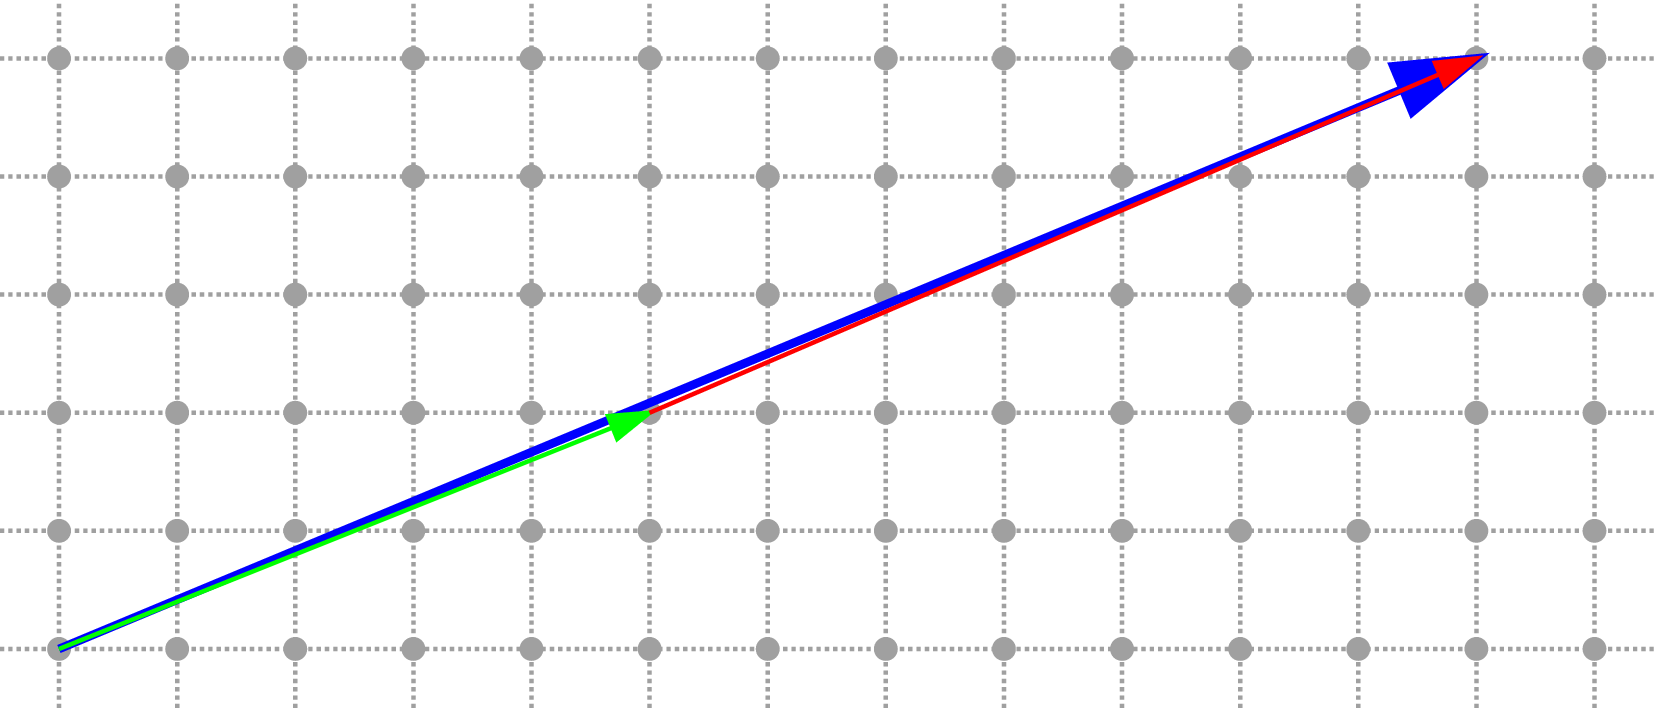
\includegraphics[width=0.45\textwidth]{split-5-12}&
    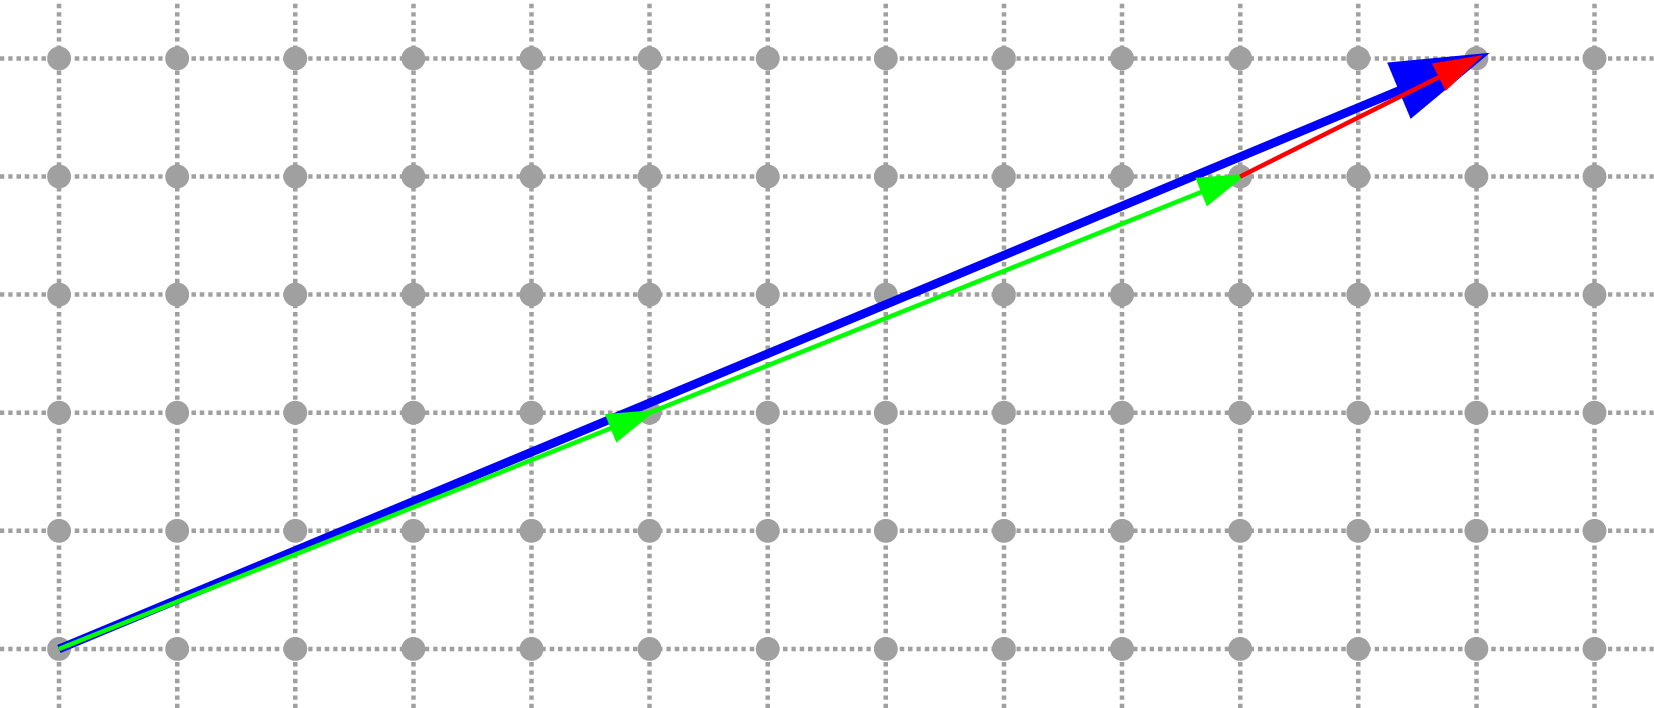
\includegraphics[width=0.45\textwidth]{splitB-5-12}\\
    split $5/12 = 2/5 \oplus 3/7$ & Berstel $5/12 = 2/5 \oplus 2/5 \oplus 1/2$ \\
  \end{tabular}

  \begin{itemize}
  \item obvious link with B�zout points, leaning points of straight lines.
  \end{itemize}
\end{frame}

%%%%%%%%%%%%%%%%%%%%%%%%%%%%%%%%%%%%%%%%%%%%%%%%%%%%%%%%%%%%%%%%%%%%%%%%%%%%%%%
\section{Patterns, straightness}
%%%%%%%%%%%%%%%%%%%%%%%%%%%%%%%%%%%%%%%%%%%%%%%%%%%%%%%%%%%%%%%%%%%%%%%%%%%%%%%


%------------------------------------------------------------------------------
\begin{frame}
  \frametitle{Digital straight segments as Patterns}

  \only<1>{
  \begin{definition}[Pattern]%[\Cite{Christoffel, 1875}]
    Freeman chain code between two consecutive upper leaning points of a digital
    straight line
  \end{definition}

    \begin{center}
      \begin{tabular}{cc}
        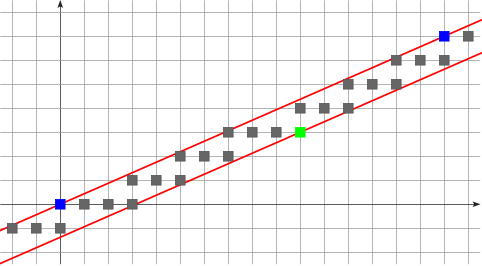
\includegraphics[width=4.2cm]{Images/pattern_dsl.png} &
        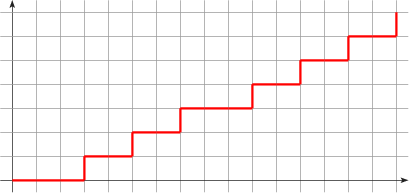
\includegraphics[width=4cm]{Images/pattern4.png} \\
        DSL( 7, 16, 0 ) & 00010010010001001001001\\
      \end{tabular}
    \end{center}
  $=$ Christoffel words [\Cite{Christoffel, 1875}]
  }

  \only<2-3>{ 
    {\small Recursive formula \Cite{Berstel, 96}
      (also splitting formula \Cite{Bruckstein \ldots})}

    \[ \frac{7}{16} = [0, 2, 3, 2] \]

    \begin{tabular}{ccccc}
      $E( [0, 2, 3, \alertred{2}] )$ & = & 
      $E( [0, 2, 3 ] )^\alertred{2}$ & $E( [0, 2 ] )$ \\
      $00010010010001001001001$ & = & $(0001001001)^\alertred{2}$ & $001$ \\
      \raisebox{-1.5em}{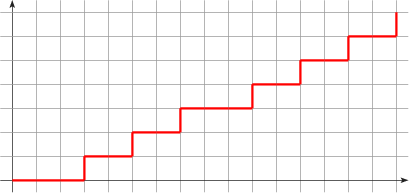
\includegraphics[width=4cm]{Images/pattern4.png}} & = & 
      $\left( \raisebox{-1em}{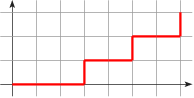
\includegraphics[width=2cm]{Images/pattern3.png}} \right)^\alertred{2}$ &
      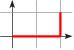
\includegraphics[width=0.75cm]{Images/pattern2.png} \\

      \only<3>{
      $E( [0, 2, \alertred{3}] )$ & = & 
      $E( [ 0 ] )$ & $E( [0, 2 ] )^\alertred{3}$ \\
      $0001001001$ & = & $0$ & $(001)^\alertred{3}$ \\
      \raisebox{-1em}{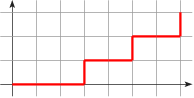
\includegraphics[width=2cm]{Images/pattern3.png}} & = & 
      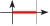
\includegraphics[width=0.5cm]{Images/pattern1.png} &
      $\left( \raisebox{0em}{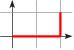
\includegraphics[width=0.75cm]{Images/pattern2.png}} \right)^\alertred{3}$ \\
      }
    \end{tabular}
  }
\end{frame}
%------------------------------------------------------------------------------

%------------------------------------------------------------------------------
\begin{frame}[fragile]
  \frametitle{Patterns in DGtal}

  {\small
  Class \href{http://liris.cnrs.fr/dgtal/doc/nightly/classDGtal_1_1Pattern.html}{\texttt{\alert{Pattern}$<$Fraction$>$}}
  }

  \lstset{language=c++, numbers=left, tabsize=2, frame=single, breaklines=true, basicstyle=\ttfamily\tiny,
     numberstyle=\tiny\ttfamily, framexleftmargin=13mm, xleftmargin=12mm,keywordstyle=\color{blue}\bfseries,%
     commentstyle=\sffamily\color{red}}
  \lstset{emph={rE, rEs,Pattern},emphstyle=\color{MyGreen}}
  
  \begin{lstlisting}
    ...
  typedef LighterSternBrocot<int32_t,int32_t> SB; // Stern-Brocot tree
  typedef SB::Fraction Fraction; // the type for fractions
  typedef Pattern<Fraction> MyPattern; // the type for patterns

  DGtal::int32_t p = atoi( argv[ 1 ] );
  DGtal::int32_t q = atoi( argv[ 2 ] );
  MyPattern pattern( p, q );
   
  bool sub = ( argc > 3 ) && ( std::string( argv[ 3 ] ) == "SUB" );
  cout << ( ! sub ? pattern.rE() : pattern.rEs( "(|)" ) ) << endl;
  \end{lstlisting}

  \lstset{language=bash, numbers=left, tabsize=2, frame=single, breaklines=true, basicstyle=\ttfamily\tiny,
     numberstyle=\tiny\ttfamily, framexleftmargin=13mm, xleftmargin=12mm,keywordstyle=\color{blue}\bfseries,%
     commentstyle=\sffamily\color{red}}

   \begin{lstlisting}
bash> ./examples/math/arithmetic/pattern 11 17 
0010010100101001010010100101
bash> ./examples/math/arithmetic/pattern 11 17 SUB
((00|1)|(0|0101)(0|0101)(0|0101)(0|0101)(0|0101))
   \end{lstlisting}

  
\begin{itemize}
\item[+] positions of leaning points
\item[+] \small greatest included subpattern given some $[AB]$
\item[+] \small smallest covering subpattern given some $[AB]$
\end{itemize}


\end{frame}
%------------------------------------------------------------------------------

%------------------------------------------------------------------------------
\begin{frame}[fragile]
  \frametitle{Digital straight lines}

  \centerline{
    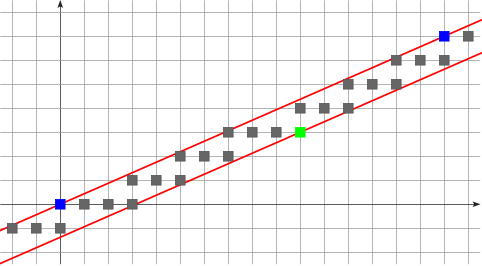
\includegraphics[width=0.3\textwidth]{Images/pattern_dsl}
  }

  {\small Class
    \href{http://liris.cnrs.fr/dgtal/doc/nightly/classDGtal_1_1StandardDSLQ0.html}{\texttt{\alert{StandardDSLQ0}$<$Fraction$>$}}
  }, characteristics $(a,b,\mu)$

  \lstset{language=c++, numbers=left, tabsize=2, frame=single, breaklines=true, basicstyle=\ttfamily\tiny,
     numberstyle=\tiny\ttfamily, framexleftmargin=13mm, xleftmargin=12mm,keywordstyle=\color{blue}\bfseries,%
     commentstyle=\sffamily\color{red}}
  \lstset{emph={StandardDSLQ0},emphstyle=\color{MyGreen}}
  
  \begin{lstlisting}
    #include "DGtal/math/arithmetic/StandardDSLQ0.h"
    ...
    typedef ... Fraction;
    typedef StandardDSLQ0<Fraction> DSL;
    ...
    DSL D( 7, 16, 0 ); // (a, b, mu)
  \end{lstlisting}

  \begin{itemize}
  \item \small get characteristics: {\tt a(), b(), mu(), mup()}
  \item \small get slope {\tt slope()} and pattern {\tt pattern()}
  \item \small get first upper leaning point in quadrant {\tt U()}, next lower {\tt L()}
  \item \small get points from given abscissa or ordinate {\tt lowestY( x )}, ...
  \end{itemize}
\end{frame}

%------------------------------------------------------------------------------
\begin{frame}[fragile]
  \frametitle{Digital straight lines can be enumerated}


  \centerline{
    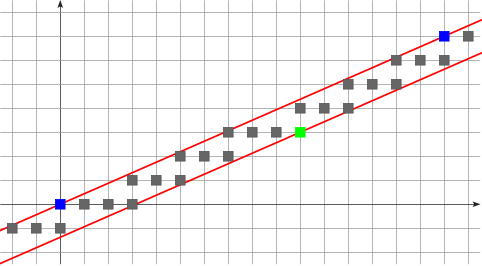
\includegraphics[width=0.3\textwidth]{Images/pattern_dsl}
    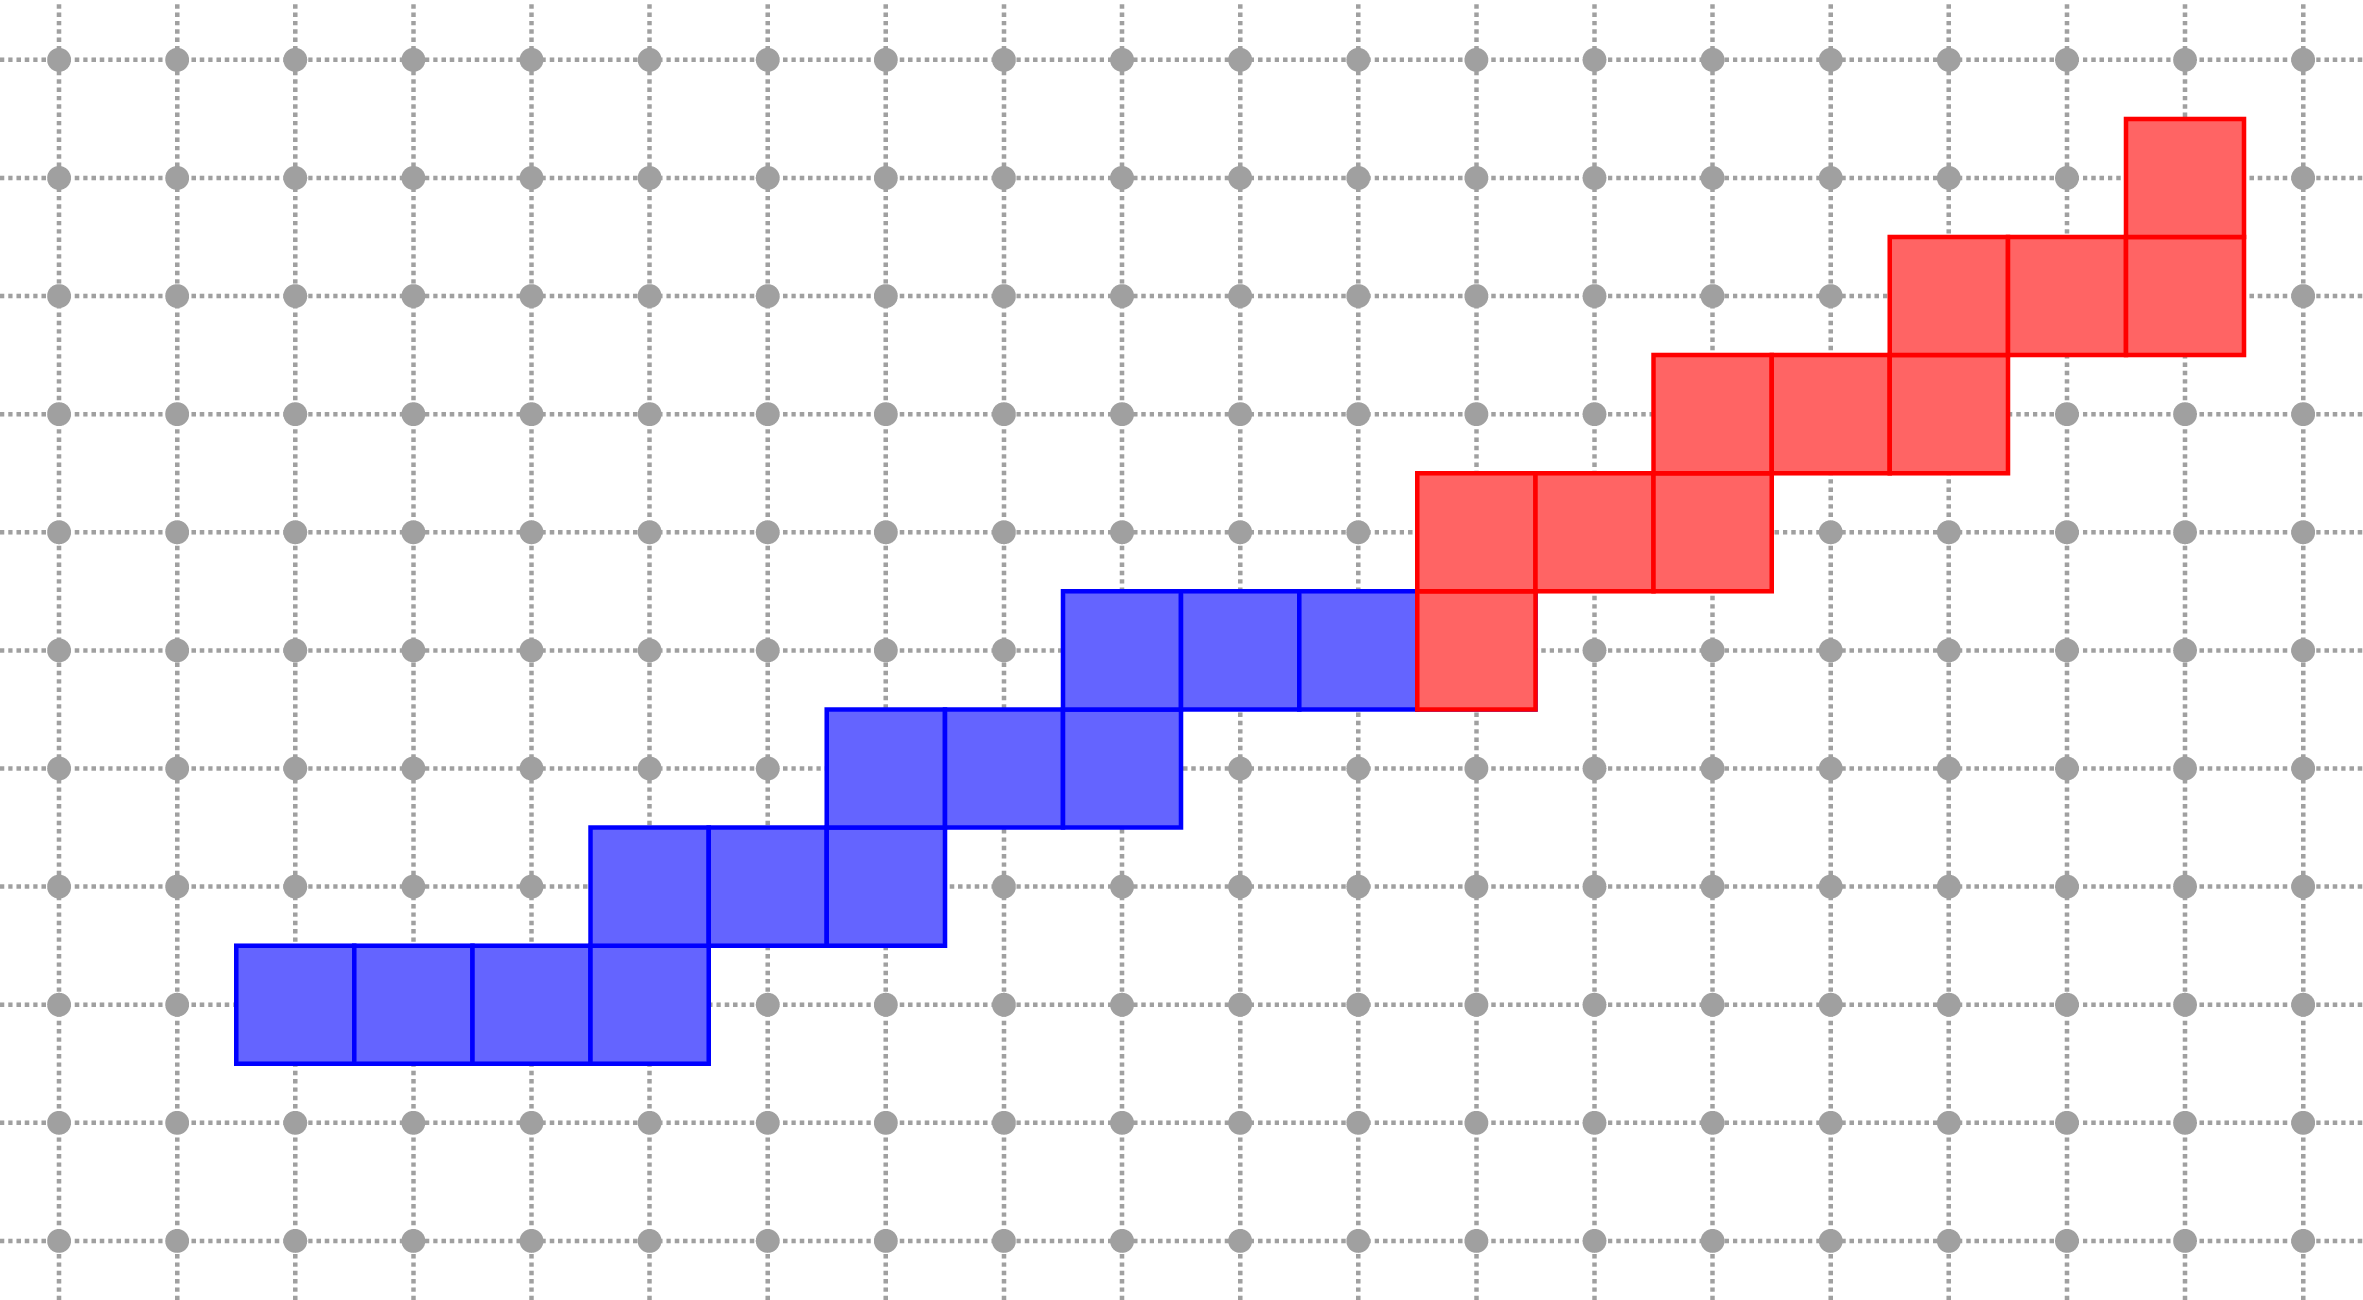
\includegraphics[width=0.3\textwidth]{Images/dsl}
  }

  \lstset{language=c++, numbers=left, tabsize=2, frame=single, breaklines=true, basicstyle=\ttfamily\tiny,
     numberstyle=\tiny\ttfamily, framexleftmargin=13mm, xleftmargin=12mm,keywordstyle=\color{blue}\bfseries,%
     commentstyle=\sffamily\color{red}}
  \lstset{emph={StandardDSLQ0,L,U,begin,end,v},emphstyle=\color{MyGreen}}
  
  \begin{lstlisting}
  typedef StandardDSLQ0<Fraction> DSL;
  typedef DSL::ConstIterator ConstIterator;
  DSL D( 7, 16, 0 ); // (a, b, mu)
  board << CustomStyle( plow.className(), // in blue
                        new CustomColors( Color(0,0,255),
                                          Color(100,100,255) ) );
  // segment [UL[                                          
  for ( ConstIterator it = D.begin( D.U() ),
          itend = D.end( D.L() ); it != itend; ++it )
    board << *it;
  board << CustomStyle( plow.className(), // in red
                        new CustomColors( Color(255,0,0),
                                          Color(255,100,100) ) );
  // segment [LU'[                                          
  for ( ConstIterator it = D.begin( D.L() ),
          itend = D.end( D.U() + D.v() ); it != itend; ++it )
    board << *it;
  \end{lstlisting}

  \begin{itemize}
  \item \small A DSL is also a model of Class
    \href{http://liris.cnrs.fr/dgtal/doc/nightly/structDGtal_1_1CPointPredicate.html}{\texttt{\alert{CPointPredicate}}}
  \end{itemize}
\end{frame}

%------------------------------------------------------------------------------
\begin{frame}[fragile]
  \frametitle{Fast extraction of subsegments}

  \small
  Knowing a DSL $D$, what are the characteristics of a subsegment $[A,B]$ ?

  \scriptsize
  \begin{itemize}
    \item standard recognition of the segment $[A,B]$ e.g. \Cite{Debled, Reveilles 1995}\\
      $\Rightarrow$ linear in its length
    \item {\tt D.smartDSS(...)} recognition by going top-down the Stern-Brocot tree. \Cite{Said, L. 2009} \\
      $\Rightarrow$ linear in the sum of the quotients of output slope
    \item {\tt D.reversedSmartDSS(...)} recognition by going bottom-up the Stern-Brocot tree.  \Cite{Said, L. 2010} \\
      $\Rightarrow$ linear in the depth of output slope
  \end{itemize}

\newcommand{\ALG}[1]{\textbf{#1}}

\begin{center}
\begin{tabular}{|r|r|r|r|r|} \cline{2-5}
\multicolumn{1}{c}{\mbox{$\;$}} & \multicolumn{4}{|c|}{Speed-up factor wrt \ALG{ArithmeticDSS}} \\ \cline{2-5}
\multicolumn{1}{c}{\mbox{$\;$}} & \multicolumn{2}{|c|}{\ALG{SmartDSS}} & \multicolumn{2}{|c|}{\ALG{ReversedSmartDSS}} \\ \hline
$N$ & $M=N/10$ & $M=N/2$& $M=N/10$ & $M=N/2$\\ \hline \hline
30 & 1,2 & 1,5 & 1,1 & 1,4 \\
400 & 2,3 & 6,8 & 2,2 & 6,8 \\
1600 & 6,7 & 26,9 & 6,3 & 27,7 \\
25600 & 70,9 & 378,3 & 75,5 & 441,9 \\
409600 & 2195,0 & 22274,8 & 2574,1 & 27239,4 \\ \hline
\end{tabular}
\end{center}

\end{frame}


\end{document}
